% Secciones de la Etapa 2 (borrador). Reemplazan "Proposed Experimental Methodology" del artículo de la Etapa 1.
% Requiere el macro \todo{...} (definido en borrador.tex). Las tablas y figuras salen de ../results/report/
% (scripts/make_report.py): si cambian los resultados se regenera ese informe y se recompila.

\section{Experimental Methodology}
\label{sec:method2}

\subsection{Data and Partitions}
We use the Kaggle ``Emotions'' dataset, a derivative of CARER \cite{saravia2018carer}, with six classes (sadness, joy, love, anger, fear, surprise). The downloaded file has 416,809 rows, and its SHA-256 digest is verified on every download. Cleaning has one purpose: no text, and no near copy of a text, may appear in two partitions. Texts are normalized only to compare them, and the original text is the one used for training. Rows whose normalized text appears with different labels are removed entirely (44,650 rows, 22,295 distinct texts), because neither label can be trusted. Exact duplicates with the same label are collapsed to one copy (632 copies removed). Near duplicates are detected with TF-IDF cosine similarity and a 0.90 threshold, over candidate pairs generated from rare terms: 5,536 pairs form 3,220 groups of two or more texts, 16 of them with mixed labels. Groups are not removed, because each group is assigned to a single partition. The result has 371,527 rows. Cleaning removed proportionally more minority-class rows (about 34\% of surprise, 29\% of love, and 17\% of fear relative to the original file), so the final distribution is sadness 31.2\%, joy 34.8\%, love 6.6\%, anger 14.1\%, fear 10.7\%, and surprise 2.7\%. We also found that every text is lowercase and has no punctuation or apostrophes (0.000\% of texts contain either), so, contrary to our Stage~1 plan, case and punctuation cues are not available to any model.

The partition is a stratified, group-aware 10-fold split (\texttt{StratifiedGroupKFold}, seed 42) over the near-duplicate groups: fold 0 is the test set (37,153 texts), fold 1 is validation (37,154), and the remaining eight folds are training (297,220). Automatic checks must pass before any training: empty intersections, no repeated normalized text across partitions, no split group, and class proportions within $\pm 0.5$ percentage points of the global ones. A stratified sample of 10,000 validation texts (the selection set) drives early stopping. All models train on the same stratified subset $S$ of 32,000 training texts (11\% of the training fold). Its size was set by the slowest model (Gemma 4 E2B, three seeds, three epochs, about eight hours) so that every model sees exactly the same data. The test set is scored once per final configuration.

\subsection{Models}
Table~\ref{tab:taxonomy2} lists the eight models and the four controlled pairs that isolate one factor each: scale in encoders (DistilBERT vs. BERT-base), scale in decoders (Qwen2.5-0.5B vs. Qwen2.5-1.5B), family (Qwen2.5-1.5B vs. Gemma 4 E2B), and training objective (Qwen2.5-1.5B vs. DeepSeek-R1-Distill-Qwen-1.5B). Gemma 4 E4B, part of the Stage~1 plan, was dropped: even in 4-bit it needs an estimated 8.77~GB (its embedding tables, about 6.5~GB, are not quantized by bitsandbytes), which leaves no room for activations and optimizer state in 10~GB, and running it unquantized on another machine would confound scale with quantization.

\begin{table}[htbp]
\centering
\caption{Models and the controlled pairs they form.}
\label{tab:taxonomy2}
\footnotesize
\begin{tabular}{@{}>{\raggedright\arraybackslash}p{0.44\linewidth}>{\raggedright\arraybackslash}p{0.17\linewidth}>{\raggedright\arraybackslash}p{0.3\linewidth}@{}}
\toprule
\textbf{Model} & \textbf{Family} & \textbf{Pair (factor)} \\
\midrule
Dummy (two strategies), TF-IDF + LogReg & Baselines & Trivial and classical reference \\
BiLSTM + GloVe & Recurrent & Recurrent baseline \\
DistilBERT & Encoder & vs. BERT-base (scale) \\
BERT-base & Encoder & vs. DistilBERT (scale) \\
Qwen2.5-0.5B & Decoder & vs. Qwen2.5-1.5B (scale) \\
Qwen2.5-1.5B & Decoder & vs. the other three decoders \\
Gemma 4 E2B & Decoder & vs. Qwen2.5-1.5B (family) \\
DeepSeek-R1-Distill-Qwen-1.5B & Decoder & vs. Qwen2.5-1.5B (objective) \\
\bottomrule
\end{tabular}
\end{table}

\textit{Baselines.} The trivial baselines, fitted on $S$, predict the most frequent class or sample from the class frequencies (three seeds for the sampling one). The classical baseline is TF-IDF with word 1--2-grams and multinomial logistic regression with class weights, fitted on training data only. The recurrent baseline is a BiLSTM (hidden size 128, dropout 0.3) over a vocabulary built from training texts only (21,897 entries), with frozen GloVe 300-dimensional vectors \cite{pennington2014glove} \todo{Fran: confirm the exact GloVe file used (6B tokens?)}.

\textit{Encoders} are fully fine-tuned with the sequence-classification head of the Transformers library over the [CLS] representation. \textit{Decoders} use a sequence-classification head over the last non-padding token (a manual linear head with the same design for Gemma 4, because the library has no such class), with no text generation and no prompt template: the raw text goes in and six logits come out. All decoders use QLoRA with 4-bit NormalFloat base weights and identical adapters: rank $r=16$, $\alpha=32$, dropout 0.05, on the $W_q, W_k, W_v, W_o$ projections (for Gemma 4, only in the language layers), with the head trained in full. This differs from the Stage~1 plan, which gave DeepSeek extra feed-forward modules; we use identical adapters so the pair isolates one factor. One factor remains confounded: DeepSeek-R1-Distill-Qwen-1.5B was distilled into Qwen2.5-Math-1.5B, not into Qwen2.5-1.5B \cite{deepseekai2025r1}, so that pair varies the base model as well as the training objective.

\subsection{Training Protocol and Hyperparameter Search}
All neural models use AdamW (weight decay 0.01), 6\% linear warmup followed by linear decay, gradient clipping at 1.0, an effective batch of 32 (with gradient accumulation), and inputs truncated to 64 tokens (the worst tokenizer truncates 0.15\% of texts). The loss is cross-entropy with class weights $w_c = N/(K n_c)$ computed on $S$; evaluation metrics are never weighted. Models train for at most three epochs (ten for the BiLSTM), are evaluated on the selection set every quarter epoch, and stop early when Macro-F1 does not improve in three evaluations; the best checkpoint is restored. Every neural model is trained with seeds 42, 1337, and 2026, which control head initialization, data order, and dropout but not the partition. Precision is bf16 on the RTX 3080 and fp16 on the RTX 2060; the BiLSTM and TF-IDF run on CPU.

Hyperparameters are searched on the selection set only, never on the test set (Table~\ref{tab:hpo}). The decoder search ran on 20\% of $S$ for one epoch, changing one factor at a time around the center point (learning rate in $\{10^{-4}, 2\times10^{-4}, 3\times10^{-4}\}$, rank in $\{8, 16, 32\}$ with $\alpha = 2r$); learning rate $3\times10^{-4}$ and rank 32 collapsed to a single predicted class. The configuration chosen on Qwen2.5-1.5B is reused for every decoder, and the encoder learning rate chosen on BERT-base is reused for DistilBERT. The winners for encoders, TF-IDF, and the BiLSTM sit at the edge of their grids, so we cannot claim they are the true optimum.

\begin{table*}[t]
\centering
\caption{Hyperparameter search results (selection-set Macro-F1, one seed). Decoders were tuned on 20\% of $S$ for one epoch; the other families on the full $S$ (BiLSTM on 20\% of $S$).}
\label{tab:hpo}
\small
% Generado por scripts/make_report.py. No editar a mano.
\begin{tabular}{@{}llrr@{}}
\toprule
Family (tuned on) & Selected configuration & Trials & Val. Macro-F1 \\
\midrule
BiLSTM & lr = $3\times10^{-3}$, hidden = 128, dropout = 0.3 & 8 & 0.9475 \\
Decoders (Qwen2.5-1.5B) & lr = $2\times10^{-4}$, LoRA $r$ = 16 & 5 & 0.8739 \\
Encoders (BERT-base) & lr = $5\times10^{-5}$ & 3 & 0.9921 \\
TF-IDF & $C$ = 10.0, n-gram = 1--2 & 6 & 0.9480 \\
\bottomrule
\end{tabular}

\end{table*}

\subsection{Evaluation and Statistics}
Macro-F1 over the six classes is the primary metric, with per-class F1 and the $6\times6$ confusion matrix; we report the mean and sample standard deviation over three seeds (TF-IDF and the most-frequent baseline are deterministic and have one run). Controlled pairs are compared with a paired bootstrap on the test set: 1,000 resamples of the same text ids for both models, and a 95\% percentile interval for the difference in Macro-F1, computed per seed (seed $k$ of model A against seed $k$ of model B). A difference counts as systematic only if the interval excludes zero with the same sign in all three seeds. We do not run a test over three seeds, which has no power.

\subsection{Explainability Protocol}
We explain BERT-base (seed 42) on a class-stratified sample of 600 test texts (up to 100 per class) plus 40 of its test errors for qualitative reading; DistilBERT and the decoders are not explained, which is a stated limitation. Our main method is Integrated Gradients \cite{sundararajan2017axiomatic} over the input word embeddings, with a [PAD] baseline and 64 Gauss-Legendre steps, contrasted with the last-layer [CLS] attention and attention rollout \cite{abnar2020quantifying}. Attention is reported only as a contrast, not as an explanation by itself \cite{jain2019attention,wiegreffe2019attention}. Before interpreting any attribution we check that the attributions sum to the output difference (completeness) and that they change when the classification head or the whole model is randomized \cite{adebayo2018sanity}. Faithfulness is measured by removing, or keeping only, the $k$ most attributed words against $k$ random words \cite{deyoung2020eraser}, and attributed words are compared with class-marker words obtained by log-odds with an informative prior \cite{monroe2008fightin}. The implementation is checked by a test on tiny models trained on a synthetic corpus where the deciding word is known (\texttt{scripts/test\_xai\_toy.py}).

\section{Results and Analysis}
\label{sec:results2}

\subsection{Overall Comparison}
Table~\ref{tab:main} and Fig.~\ref{fig:macrof1} show the final results on the 37,153 test texts. BERT-base reaches the highest Macro-F1 ($0.9895 \pm 0.0005$), with DistilBERT $0.0004$ behind at 61\% of the parameters and 58\% of the training time. The top five models, two encoders and three decoders, lie within $0.0021$ Macro-F1 of each other, a range comparable to the seed-to-seed standard deviation of the decoders (0.0008 to 0.0012). The BiLSTM with GloVe follows at $0.9786 \pm 0.0028$. Gemma 4 E2B ($0.9544 \pm 0.0032$) and TF-IDF with logistic regression ($0.9493$) are clearly lower, and the trivial baselines sit at $0.1696$ (stratified) and $0.0861$ (most frequent). A linear model on word n-grams therefore comes within four points of the best model, and the task as framed here is close to saturated.

\begin{table*}[t]
\centering
\caption{Test Macro-F1 (mean $\pm$ sample standard deviation over three seeds) and cost per model. VRAM is the training peak; time is per run on the machine that trained it (RTX 2060 for encoders and Qwen2.5-0.5B, RTX 3080 for the other decoders, CPU for BiLSTM and TF-IDF), so costs are not comparable across GPUs. $^{\dagger}$Published parameter count of the base model; the harness counts each 4-bit weight pair as one element and under-reports. Both Dummy baselines were trained on $S$.}
\label{tab:main}
\small
% Generado por scripts/make_report.py. No editar a mano.
\begin{tabular}{@{}lrrrr@{}}
\toprule
Model & Macro-F1 (test) & Params & VRAM (GB) & Time (min) \\
\midrule
BERT-base & 0.9895 $\pm$ 0.0005 & 109.5M & 2.2 & 16.6 \\
DistilBERT & 0.9891 $\pm$ 0.0003 & 67.0M & 1.4 & 9.6 \\
\midrule
Qwen2.5-1.5B & 0.9887 $\pm$ 0.0012 & 1.54B$^{\dagger}$ & 2.7 & 72.7 \\
Qwen2.5-0.5B & 0.9877 $\pm$ 0.0010 & 0.49B$^{\dagger}$ & 1.2 & 85.5 \\
DeepSeek-R1-Distill-1.5B & 0.9874 $\pm$ 0.0008 & 1.54B$^{\dagger}$ & 2.7 & 79.0 \\
\midrule
BiLSTM + GloVe & 0.9786 $\pm$ 0.0028 & 7.0M & -- & 9.6 \\
\midrule
Gemma 4 E2B & 0.9544 $\pm$ 0.0032 & 5.1B$^{\dagger}$ & 9.2 & 149.4 \\
\midrule
TF-IDF + LogReg & 0.9493 & 344K & -- & 0.2 \\
\midrule
Dummy (stratified) & 0.1696 $\pm$ 0.0014 & -- & -- & $<$0.1 \\
Dummy (most frequent) & 0.0861 & -- & -- & $<$0.1 \\
\bottomrule
\end{tabular}

\end{table*}

\begin{figure}[htbp]
\centering
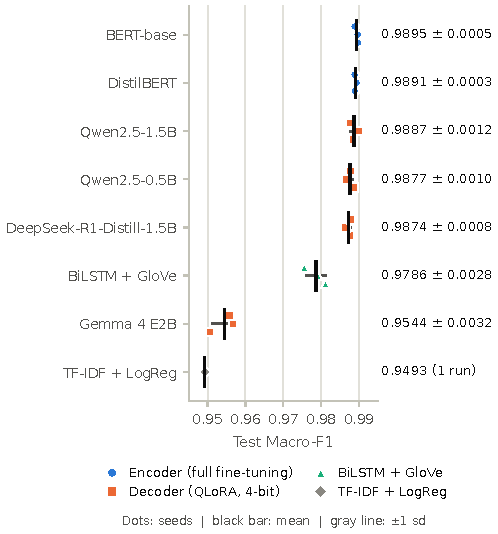
\includegraphics[width=\linewidth]{../results/report/fig_macro_f1.pdf}
\caption{Test Macro-F1 per model: points are seeds, the mark is the mean, and the line is $\pm1$ standard deviation. The Dummy baselines fall outside the plotted range (Table~\ref{tab:main}).}
\label{fig:macrof1}
\end{figure}

\subsection{Controlled Pairs}
Table~\ref{tab:pairs} reports the paired bootstrap. Qwen2.5-1.5B beats Gemma 4 E2B by $0.034$ Macro-F1 on average, and the interval excludes zero in all three seeds with the same sign: the family gap is systematic, although it includes any residual difference between our manual Gemma head and the library head used for Qwen. Between Qwen2.5-1.5B and DeepSeek-R1-Distill-Qwen-1.5B the mean difference is $0.0013$, the interval excludes zero in only one seed, and the sign changes: there is no consistent difference attributable to the training objective, and this pair is also confounded by the base model. Neither scale pair shows a consistent difference. DistilBERT trails BERT-base by $0.0004$ on average and the interval includes zero in all three seeds, so we cannot detect a difference between them. Qwen2.5-0.5B trails Qwen2.5-1.5B by $0.0010$ on average, but the interval excludes zero in only one seed (1337) and the sign changes between seeds; this pair is also confounded by precision (fp16 for the smaller model, bf16 for the larger) and by the machine that trained each.

\begin{table*}[t]
\centering
\caption{Paired bootstrap over the test set (1,000 resamples, 95\% interval, per seed): mean difference in Macro-F1 of A minus B, number of seeds whose interval excludes zero, and whether the sign is the same in all seeds.}
\label{tab:pairs}
\small
% Generado por scripts/make_report.py. No editar a mano.
\begin{tabular}{@{}lrrc@{}}
\toprule
Pair (A vs. B) & Mean $\Delta$ Macro-F1 & Seeds with CI excluding 0 & Same sign \\
\midrule
DistilBERT vs. BERT-base & -0.0004 & 0/3 & no \\
Qwen2.5-0.5B vs. Qwen2.5-1.5B & -0.0010 & 1/3 & no \\
Qwen2.5-1.5B vs. Gemma 4 E2B & +0.0343 & 3/3 & yes \\
Qwen2.5-1.5B vs. DeepSeek-R1-Distill-1.5B & +0.0013 & 1/3 & no \\
\bottomrule
\end{tabular}

\end{table*}

\subsection{Per-Class Results and Error Analysis}
Table~\ref{tab:perclass} shows that for every neural model the three lowest F1 scores are surprise, fear, and anger, while love, despite being a minority class (6.6\%), is among the easiest; Gemma 4 E2B loses most on surprise ($0.9222$ against $0.9798$ for Qwen2.5-1.5B). We analyzed the errors of all eight models; a text counts as an error of a model if it fails it in most of the model's seeds. The five best models make between 258 (BERT-base, 0.69\%) and 335 (DeepSeek-R1-Distill-Qwen-1.5B, 0.90\%) such errors and share many of them: the Jaccard index is 0.62 between the two encoders and 0.54 between Qwen2.5-1.5B and DeepSeek-R1-Distill-Qwen-1.5B. Gemma 4 E2B (1,375 errors, 3.70\%) and TF-IDF (1,620, 4.36\%) are different: 80.1\% and 76.9\% of their errors are made by no other model, against 2\% to 8\% for the five best, which points to a model limitation more than to a property of the data. At the other end, 64 texts (0.17\%) are misclassified by all eight models, and for 22 of them all eight predict the same wrong class. The corpus is made almost entirely of tweets built around ``feel'' (98.5\% of the test texts). The 562 texts without that word (1.5\%) have error rates of 27\% to 35\% for the five best models (46\% for the BiLSTM and 45\% for TF-IDF), against 0.4\% to 0.5\% for the rest; they hold 59\% to 61\% of the errors of the five best models and 86\% of the consensus errors. We read the consensus errors as ambiguous or possibly mislabeled texts, but that is a hypothesis: a manual audit of 30 sampled consensus errors is pending \todo{Audit the 30 texts listed in section 5 of results/errors/cross\_model.md and report the A/B/C counts, or remove the label-noise reading.}

\begin{table*}[t]
\centering
\caption{Per-class F1 on the test set (mean over three seeds).}
\label{tab:perclass}
\small
% Generado por scripts/make_report.py. No editar a mano.
\begin{tabular}{@{}lrrrrrr@{}}
\toprule
Model & Sadness & Joy & Love & Anger & Fear & Surprise \\
\midrule
BERT-base & 0.9942 & 0.9956 & 0.9954 & 0.9871 & 0.9850 & 0.9795 \\
DistilBERT & 0.9941 & 0.9949 & 0.9948 & 0.9863 & 0.9844 & 0.9800 \\
Qwen2.5-1.5B & 0.9946 & 0.9944 & 0.9962 & 0.9850 & 0.9821 & 0.9798 \\
Qwen2.5-0.5B & 0.9932 & 0.9933 & 0.9958 & 0.9828 & 0.9829 & 0.9780 \\
DeepSeek-R1-Distill-1.5B & 0.9931 & 0.9932 & 0.9956 & 0.9835 & 0.9797 & 0.9791 \\
BiLSTM + GloVe & 0.9834 & 0.9852 & 0.9864 & 0.9728 & 0.9751 & 0.9691 \\
Gemma 4 E2B & 0.9753 & 0.9706 & 0.9687 & 0.9466 & 0.9430 & 0.9222 \\
TF-IDF + LogReg & 0.9607 & 0.9641 & 0.9449 & 0.9460 & 0.9454 & 0.9346 \\
Dummy (stratified) & 0.3149 & 0.3509 & 0.0699 & 0.1455 & 0.1085 & 0.0282 \\
Dummy (most frequent) & 0.0000 & 0.5166 & 0.0000 & 0.0000 & 0.0000 & 0.0000 \\
\bottomrule
\end{tabular}

\end{table*}

\subsection{Cost}
Fig.~\ref{fig:cost} plots Macro-F1 against training VRAM and parameters. QLoRA trains between 2.2M and 5.4M parameters (below 0.5\% of the base model), and the decoders peak at 1.2 to 2.7~GB of training VRAM, except Gemma 4 E2B, which needs 9.2~GB and 149 minutes per run for the lowest decoder accuracy. Encoders reach the best Macro-F1 at 1.4 to 2.2~GB and under 17 minutes per run. These numbers come from different GPUs, so we report them per model and do not compare them across machines; we did not measure inference latency.

\begin{figure*}[t]
\centering
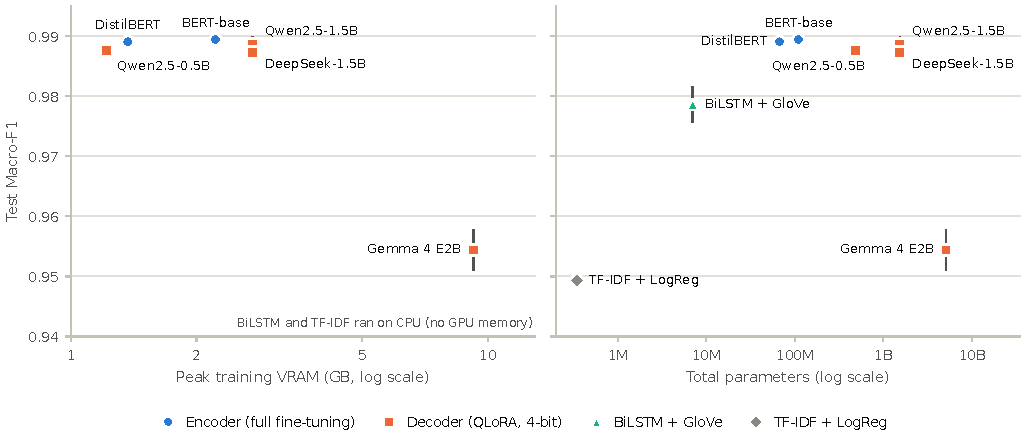
\includegraphics[width=0.8\textwidth]{../results/report/fig_cost_perf.pdf}
\caption{Macro-F1 against training VRAM (left) and total parameters (right). Costs come from different GPUs and are descriptive only.}
\label{fig:cost}
\end{figure*}

\subsection{Explainability of BERT-base}
\label{sec:xai}
We explain BERT-base (seed 42) on 600 test texts sampled by class and on 40 of the 287 errors that this run makes on the test set. The sample is small and the intervals (1.96 standard errors) cover the sampling of texts, not the seed.

\textit{Sanity checks.} Predictions recomputed in fp32 agree with the stored ones in all 640 texts. The completeness error of Integrated Gradients is 1.6\% on average (median 0.2\%, 95th percentile 6.4\%), below our 5\% threshold. Randomizing the whole model removes the agreement with the attributions of the trained model (mean Spearman $\rho=-0.05$, same top word in 4\% of texts). Randomizing only the classification head leaves more agreement in the top word (20\%) although the rank correlation is again near zero ($\rho=-0.12$); this is plausible because the fine-tuned encoder still carries the emotion cues.

\textit{Faithfulness.} Fig.~\ref{fig:faith} compares the methods against random words. Removing the single word with the most attribution changes the predicted class in 75.0\% of the texts and lowers the probability of that class by 0.75 on average, whereas removing one random word changes it in 7.3\% and lowers it by 0.07; with five words the drops are 0.89 and 0.27. Keeping only the top word preserves the decision in 98.5\% of the texts (99.8\% with three words). Attention is much less faithful: removing the top word of the last-layer [CLS] attention lowers the probability by 0.45, and by 0.17 for rollout, which is barely above random. The average drop over $k$ (AOPC \cite{deyoung2020eraser}) is 0.835 for Integrated Gradients, 0.632 for [CLS] attention, 0.363 for rollout, and 0.165 for random words. Removing a word by masking it is not the same as deleting it, since the model never saw such texts in training; this is why random words are the control.

\begin{figure*}[t]
\centering
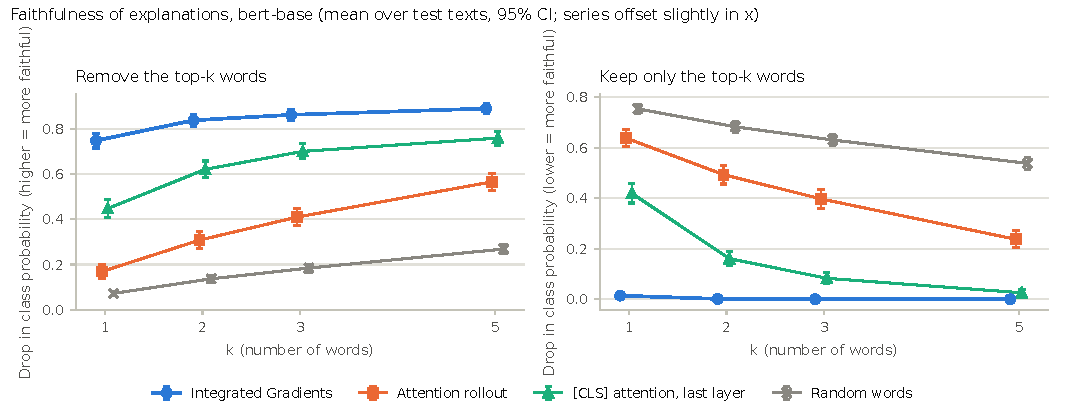
\includegraphics[width=0.85\textwidth]{../results/xai/bert-base/seed_42/fig_xai_faithfulness.pdf}
\caption{Faithfulness of the explanations of BERT-base (seed 42, 600 test texts, 95\% interval). Left: drop in the probability of the predicted class when the $k$ most attributed words are removed. Right: drop when only those $k$ words are kept.}
\label{fig:faith}
\end{figure*}

\textit{Which words the model uses.} The top word of Integrated Gradients is a class-marker word (among the 50 words with the highest log-odds of the predicted class in $S$) in 77.5\% of the texts, against 11.6\% for a random word, 46.2\% for [CLS] attention, and 19.8\% for rollout. It is never a stopword (random words are, in 53.4\%) and it is the word ``feel'' itself in only 2.5\% of the texts; in 95\% of them it comes after the first ``feel'' phrase, so the model mostly reads what follows it. Aggregated over the sample, the most attributed words for love, anger, fear, and surprise are markers (tender, gentle; irritated, insulted; intimidated, afraid; amazed, shocked), while for sadness and joy the aggregate is led by frequent words such as ``feel'' and ``i''. Integrated Gradients and rollout share the top word in 21.5\% of the texts (mean $\rho=0.17$) and Integrated Gradients and [CLS] attention in 51.8\% ($\rho=0.27$). In the last layer, 20.2\% of the [CLS] attention falls on [CLS] and [SEP] (59.7\% for rollout), one more reason to read raw attention with care.

\textit{Errors.} In several of the errors we inspected, the wrong class is driven by one strong emotion word that competes with another. In ``i wasnt feeling that horny just annoyed about work\ldots'' (true class love, predicted anger with probability 0.99), ``annoyed'' pushes toward anger with $+4.48$ and ``horny'' toward love with $+3.82$. In ``i feel so robbed of such a precious life gift'' (true class joy, predicted sadness), ``robbed'' gives $+8.23$ toward sadness and ``precious'' $+7.10$ toward joy. Such texts carry two opposing cues, which fits the hypothesis of ambiguous labels but does not prove it; more examples are in \texttt{examples.html}, next to the other explainability outputs in the repository.

\textit{Reading.} BERT-base decides with very few emotion words placed after ``feel'', and Integrated Gradients flags them faithfully. This is coherent with a TF-IDF model already reaching 0.9493 and with the lexical regularity of the corpus, but it does not show that the model understands emotion. Attributions describe the model, not the cause of the emotion in the text. They depend on a single baseline ([PAD]); other baselines might split the credit differently, and we did not test them.

\section{Limitations}
\label{sec:limits2}
The training subset $S$ is 11\% of the training fold, so the results describe a low-data regime and we did not run a learning curve. The hyperparameter search covers one model per family and its winners for encoders, TF-IDF, and the BiLSTM sit at the grid edge; the decoder search used one epoch, which favors high learning rates. Our learning rate for decoders ($2\times10^{-4}$) lies close to the instability region (rates of $3\times10^{-4}$ and rank 32 collapsed in the search), although none of the twelve final decoder runs collapsed. Machines differ in precision (fp16 on the RTX 2060, bf16 on the RTX 3080), which confounds the Qwen2.5-0.5B vs. 1.5B pair, and costs are not comparable across GPUs. Parameter counts of quantized decoders come from published figures, because the harness under-counts them. The runs of one team member did not record the commit hash. The dataset is almost entirely ``i feel \dots'' tweets, lowercase and unpunctuated, so results may not transfer to other registers, and top models differ by less than the noise of a three-seed estimate. Finally, explainability covers only BERT-base, one seed (42), a sample of 600 texts, and a single [PAD] baseline for Integrated Gradients.
